\documentclass{mywork}
\blattanadrei

\begin{document}

	\setcounter{section}{1}
	\begin{aufgabe}~

		Man sieht anhand von Aufgabe 1.2 b), dass die durch $\Re(z)=\lambda$ und $\Im(z)=\my$ gegebenen Geraden für $\lambda\neq0\neq\my$ durch $f$ auf Kreise (ohne $0$) abgebildet werden und für $\lambda=0=\my$ auf Geraden (ohne $0$).

		Es gilt zunächst mit $z=\lambda + i\my$:
		\[
			f(z) = \f 1z = \f 1{\lambda+\my i} = \f {\lambda -\my i}{\lambda^2+\my^2}= \f{\lambda}{\lambda^2+\my^2} - \f{\my}{\lambda^2+\my^2}i
		\]
		Unabhängig davon, ob wir $M_\lambda$, oder $N_\my$ betrachten, ergibt sich im Fall $z\neq 0$ durch Einsetzen in die Kreisgleichung:
		\begin{align*}
			\left(\f \lambda{\lambda^2+\my^2}-a\right)^2 + \left(\f \my{\lambda^2+\my^2}-b\right)^2&=r^2\\
			   \f 1{\lambda^2+\my^2} - \f {2\lambda a+2\my b}{\lambda^2 +\my^2} + a^2 + b^2 &= r^2\\
												(a^2+b^2-r^2)\lambda^2 + (a^2+b^2-r^2)\my^2 &= 2\lambda a + 2\my b - 1
		\end{align*}
		Für festes $\lambda\neq 0$ und beliebiges $\my$ ergibt sich automatisch $b=0$, $a=\f 1{2\lambda}$ und $r=|a|=\f1{2|\lambda|}$. Für festes $\my\neq 0$ und beliebiges $\lambda$ analog.

		Für $\lambda=0$ beschreibt $M_\lambda$ die Menge ($z=\lambda+\my i$)
		\[
			M_\lambda = \left\{\f 1{\my i} : \my\in \R\setminus \{0\}\right\} = \{ b i : b\in \R\} \setminus \{0\}
		\]
		Für $N_\my$ mit $\my=0$ analog.

		Wir können die Mengen also schreiben als
		\begin{align*}
			M_\lambda &= \begin{cases}
				\left\{a+bi\in \C : \left(a-\f 1{2\lambda}\right)^2+b^2=\f1{2|\lambda|}\right\} \setminus \{0\} & \lambda\neq 0\\
												\{bi\in \C : b\in \R\} \setminus \{0\} & \lambda=0
			\end{cases}\\
			N_\my &= \begin{cases}
				\left\{a+bi\in \C : a^2+\left(b-\f 1{2\my}\right)^2=\f1{2|\my|}\right\} \setminus \{0\} & \my\neq 0\\
												 a\in \R \setminus \{0\} & \my=0
			\end{cases}
		\end{align*}
		\begin{figure*}[h]
			\centering
			\caption{Kurvenscharen von $M_\lambda$ ($N_\my$ durch Vertauschung der Koordinatenachsen)}
			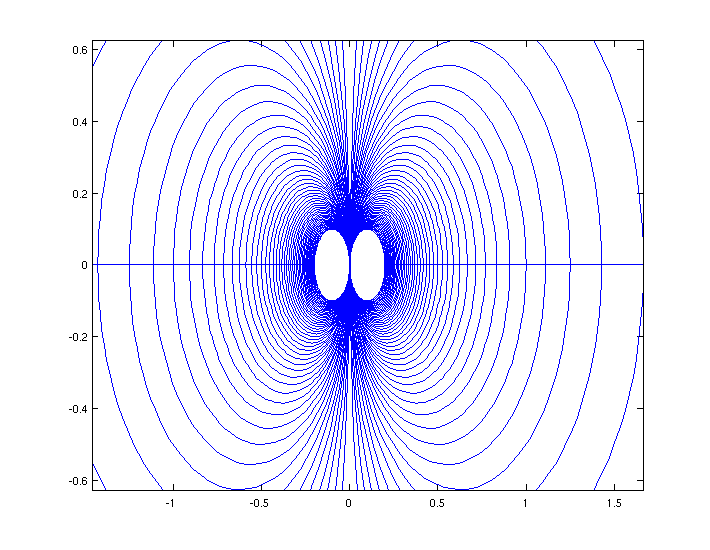
\includegraphics[scale=0.6]{ana3_1_1}
		\end{figure*}
	\end{aufgabe}


	\newpage
	\begin{aufgabe}
		\begin{enumerate}[a)]
			\item 
				\begin{seg}{Geraden und Kreise erfüllen die Gleichung}
					Zunächst wird aus der gegebenen Gleichung für $z=x+iy$ nach Umformung und Neugruppierung
					\[
						A(x^2+y^2) + (B+\_B)x + i(B-\_B)y + C = 0
					\]
					Für eine Gerade der Form $y=ax+b$, bzw. $ax -y + b = 0$ identifiziert man leicht:
					\begin{align*}
						0 = A,\qquad a = B + \_B, \qquad -1 = i(B-\_B), \qquad b = C
					\end{align*}
					Die Gerade erfüllt also mit der Wahl $A:=0, B:=\f 12(a+i), C:= b$ die gegebene Gleichung (offensichtlich auch $AC<|B|^2$).
					
					Für eine Gerade der Form $x=c$, bzw. $x-c=0$ ergibt sich ähnlich:
					\begin{align*}
						0 = A,\qquad 1 = B + \_B, \qquad 0 = i(B-\_B), \qquad -c = C
					\end{align*}
					und die Gleichung wird für $A:=0, B:=\f 12, C:= -c$ erfüllt (offensichtlich auch $AC<|B|^2$).

					Für einen Kreis mit Radius $r$ um $(a,b)$ gegeben durch die Gleichung
					\[
						(x-a)^2 + (y-b)^2 = r^2
					\]
					bzw. nach Umformung
					\[
						(x^2+y^2) - 2ax - 2by +(a^2+b^2-r^2) = 0
					\]
					identifiziert man
					\begin{align*}
						1 = A,\qquad  -2a = B + \_B, \qquad -2b = i(B-\_B), \qquad a^2+b^2-r^2 = C,
					\end{align*}
					Die Gleichung wird für $A:=1, B:= -a +bi, C:=a^2+b^2-r^2$ erfüllt.
					Außerdem gilt $AC = a^2+b^2-r^2 < a^2+b^2 = |B|^2$.
				\end{seg}
				\begin{seg}{Lösungen der Gleichung sind Geraden und Kreise}
					Sei $z=x+iy$ und durch
					\[
						Az\_z + Bz + \_B\_z + C = 0
					\]
					ein Kreis gegeben (also $A\neq 0$).
					Forme um
					\begin{align*}
						0 &= (x+iy)(x-iy) + \f BA x + \f BA yi + \f{\_B}A x - \f{\_B}Ayi B \f CA\\
					    0 &= x^2+y^2 + \f {2 \Re B}A x - \f {2\Im B}A y + \f CA\\
						  \f 1{A^2}\underbrace{\left(|B|^2 - AC\right)}_{>0}&= \left(x+\f {\Re B}A\right)^2 + \left(y-\f {\Im B}A\right)^2  
					\end{align*}
					Es ergibt sich also ein Kreis um $( -\f{\Re B}A, \f {\Im B}A)$ mit Radius $\f 1{A^2}(|B|^2-AC)$.

					Sei jetzt eine Gerade gegeben (also $A=0$).
					Dann ergibt sich nach kurzer Umformung
					\[
						(\Re B) x - (\Im B)y + C = 0
					\]
					Für $\Im B\neq 0$ ergibt sich eine Geradengleichung der Form
					\[
						y = \f {\Re B}{\Im B}x + \f C{\Im B}
					\]
					Aus $\Im B = 0$ folgt unmittelbar wegen $0=AC<|B|^2$, dass $\Re B\neq 0$ und es ergibt sich eine Gerade der Form
					\[
						x= -\f C{\Re B}
					\]
				\end{seg}
			\item
				Setze das Bild von $f$ in obige Gleichung ein.
				Wir nehmen zunächst für die Umformung $z\neq 0$ an.
				\begin{align*}
					\f A{x^2+y^2} + \f B{x+yi} + \f {\_B}{x-yi} + C &= 0\\
						   A + Bx -Byi + \_B x + \_Byi + Cx^2 +Cy^2 &= 0\\
		   \underbrace{C}_{=:A'}z\_z + \underbrace{\_B}_{=:B'}z + \underbrace{B}_{=:\_{B'}}\_z + \underbrace{A}_{=:C'} &= 0
				\end{align*}
				Offensichtlich gilt wegen $AC<|B|^2$ auch $A'C'<|B'|^2$ und es ergibt sich wieder die Gleichung, welche Kreise und Geraden beschreibt.

				Ein Kreis, der nicht $0$ enthält (also $0\neq C=A'$), wird demnach wieder auf einen Kreis abgebildet.

				Eine Gerade, die nicht $0$ enthält (also $0\neq C=A'$), wird demnach auf einen Kreis abgebildet, der die Null wegen $\hat f(\infty)=0$ enthält.

				Ein Kreis, der die $0$ enthält (also $0=C=A'$), wird demnach auf eine Gerade abgebildet ($\hat f(0)=\infty$ ist auch im Bild).

				Eine Gerade, die die $0$ enthält (also $0=C=A'$), wird demnach wieder auf eine Gerade durch $0$ ($0=A=C'$) abgebildet ($\hat f(0)=\infty$ ist auch im Bild).
		\end{enumerate}
	\end{aufgabe}

\end{document}

